\chapter{Geodesics on the Statistical Manifold}
\label{ch:geodesics}

\section{The Geometry of Probability Distributions}

In deep learning, we typically characterize the state of a neural network by its parameters $\theta \in \mathbb{R}^d$. The learning process is formulated as an optimization trajectory through this Euclidean parameter space, guided by gradients. However, a profound mismatch exists between the geometry of the map (the parameter space $\Theta$) and the geometry of the territory (the space of probability distributions $p_\theta(x)$). 

Consider the Euclidean distance between two parameter vectors, $\|\theta_1 - \theta_2\|_2$. This metric treats every parameter equally, assuming that a unit step in coordinate $\theta_i$ has the same impact as a unit step in coordinate $\theta_j$. Yet, in highly non-linear models such as deep neural networks, this is manifestly false. A small perturbation in the weights of an early layer might fundamentally alter the network's output distribution, while a massive shift in a redundant or "dead" neuron might leave the distribution completely unchanged. Measuring the distance between two networks by the Euclidean distance of their parameters is akin to measuring the distance between two cities on a Mercator projection using a standard ruler: the map severely distorts the true distances, rendering straight lines highly suboptimal.

Information geometry resolves this mismatch by recognizing that the space of probability distributions is not flat; it is a curved, Riemannian manifold known as a \textit{statistical manifold}. On this manifold, the distance between two points (distributions) is determined not by how far apart their parameter coordinates are, but by how \textit{distinguishable} the underlying distributions are from one another. 

The metric tensor that endows this space with its curvature is the Fisher Information Matrix (FIM), as introduced in Chapter 29. By equipping the parameter space with the Fisher metric, we transition from the flat, arbitrary coordinate space into a geometry that inherently respects the statistical reality of the model. Regions where the distribution is highly sensitive to parameter changes manifest as regions of high curvature or "density" on the manifold, naturally penalizing large steps in those directions. 

In any curved space, the notion of a "straight line" generalizes to a \textit{geodesic}. A geodesic is the shortest path between two points on the manifold. In the context of a statistical manifold, a geodesic represents the optimal trajectory to morph one probability distribution into another while minimizing the total accumulated "information distance." Traversing a geodesic ensures that each infinitesimal step along the path induces the smallest possible statistical change (measured locally by the Kullback-Leibler divergence). 

Understanding geodesics is critical for the foundations of deep learning. Optimization algorithms that respect the geometry of the statistical manifold—such as natural gradient descent—are fundamentally attempting to step along these geodesics. When we observe the learning dynamics of deep networks, phenomena such as "catastrophic forgetting" or "sudden representational shifts" can often be traced back to the network being forced to take highly non-geodesic paths in the distribution space simply because it is constrained to take straight paths in the parameter space. 

To fully appreciate the necessity of this geometric perspective, consider the phenomenon of "gradient starvation" or the vanishing gradient problem in deep networks. When a model's parameters are updated strictly along the Euclidean gradient of the loss, the trajectory often plunges into regions where the Fisher information is highly skewed. In these regions, the model's output distribution becomes hypersensitive to some parameters and entirely invariant to others. The Euclidean path, blindly ignorant of this curvature, takes steps that wildly perturb the distribution in some directions while making agonizingly slow progress in others. By contrast, a path aligned with the geodesics of the statistical manifold naturally scales its steps by the inverse of the Fisher metric, moving confidently through invariant regions and cautiously through hypersensitive ones. Geodesics thus represent the gold standard of learning dynamics: a perfectly paced traversal of the distribution space.

\section{Riemannian Geometry of Statistical Models}

We now formalize the notion of the statistical manifold and derive the equations governing its geodesics.

Let $\mathcal{X}$ be a measurable space (the data domain) and consider a parametric family of probability distributions $S = \{ p_\theta(x) : \theta \in \Theta \}$, where the parameter space $\Theta \subseteq \mathbb{R}^d$ is an open set. We assume that the mapping $\theta \mapsto p_\theta$ is injective and that $p_\theta(x)$ is strictly positive and sufficiently smooth with respect to $\theta$.

\begin{definition}[Statistical Manifold]
The family $S$ forms a $d$-dimensional \textit{statistical manifold} $\mathcal{M}$, where each point on the manifold corresponds to a unique probability distribution $p_\theta$, and $\theta = (\theta_1, \dots, \theta_d)$ serves as a local coordinate system.
\end{definition}

To measure lengths and angles on $\mathcal{M}$, we require a Riemannian metric tensor.

\begin{definition}[Fisher Information Metric]
The Fisher Information Matrix $I(\theta)$ acts as the canonical Riemannian metric tensor $g(\theta)$ on the statistical manifold $\mathcal{M}$. Its components are given by:
\begin{equation}
g_{ij}(\theta) = \mathbb{E}_{x \sim p_\theta} \left[ \frac{\partial \log p_\theta(x)}{\partial \theta_i} \frac{\partial \log p_\theta(x)}{\partial \theta_j} \right] = - \mathbb{E}_{x \sim p_\theta} \left[ \frac{\partial^2 \log p_\theta(x)}{\partial \theta_i \partial \theta_j} \right]
\end{equation}
The infinitesimal squared distance between $p_\theta$ and $p_{\theta + d\theta}$ is defined by the quadratic form $ds^2 = \sum_{i,j} g_{ij}(\theta) d\theta_i d\theta_j$.
\end{definition}

To rigorously justify why the Fisher Information Matrix is the correct metric tensor, we demonstrate its local equivalence to the Kullback-Leibler divergence.

\begin{theorem}[Local Equivalence of KL Divergence and Fisher Metric]
\label{thm:kl_fisher}
For two infinitesimally close distributions $p_\theta$ and $p_{\theta + \Delta \theta}$ on $\mathcal{M}$, the Kullback-Leibler divergence is locally symmetric and approximated by the Fisher Information Metric:
\begin{equation}
D_{\text{KL}}(p_\theta \parallel p_{\theta + \Delta \theta}) \approx \frac{1}{2} \sum_{i,j} g_{ij}(\theta) \Delta \theta_i \Delta \theta_j
\end{equation}
\end{theorem}

\begin{proof}
We perform a second-order Taylor expansion of the KL divergence around $\theta$. Let $\ell(\theta; x) = \log p_\theta(x)$. The divergence is given by:
\begin{equation}
D_{\text{KL}}(p_\theta \parallel p_{\theta + \Delta \theta}) = \mathbb{E}_{x \sim p_\theta} \left[ \ell(\theta; x) - \ell(\theta + \Delta \theta; x) \right]
\end{equation}
Expanding $\ell(\theta + \Delta \theta; x)$ yields:
\begin{equation}
\ell(\theta + \Delta \theta; x) \approx \ell(\theta; x) + \sum_i \frac{\partial \ell}{\partial \theta_i} \Delta \theta_i + \frac{1}{2} \sum_{i,j} \frac{\partial^2 \ell}{\partial \theta_i \partial \theta_j} \Delta \theta_i \Delta \theta_j
\end{equation}
Substituting this back into the expectation:
\begin{equation}
D_{\text{KL}}(p_\theta \parallel p_{\theta + \Delta \theta}) \approx - \sum_i \Delta \theta_i \mathbb{E}_{x \sim p_\theta} \left[ \frac{\partial \ell}{\partial \theta_i} \right] - \frac{1}{2} \sum_{i,j} \Delta \theta_i \Delta \theta_j \mathbb{E}_{x \sim p_\theta} \left[ \frac{\partial^2 \ell}{\partial \theta_i \partial \theta_j} \right]
\end{equation}
The expectation of the score function is identically zero:
\begin{equation}
\mathbb{E}_{x \sim p_\theta} \left[ \frac{\partial \ell}{\partial \theta_i} \right] = \int p_\theta(x) \frac{\partial \log p_\theta(x)}{\partial \theta_i} dx = \int \frac{\partial p_\theta(x)}{\partial \theta_i} dx = \frac{\partial}{\partial \theta_i} \int p_\theta(x) dx = \frac{\partial}{\partial \theta_i} (1) = 0
\end{equation}
The remaining term is exactly the definition of the Fisher Information Matrix, multiplied by $\frac{1}{2}$:
\begin{equation}
D_{\text{KL}}(p_\theta \parallel p_{\theta + \Delta \theta}) \approx \frac{1}{2} \sum_{i,j} g_{ij}(\theta) \Delta \theta_i \Delta \theta_j
\end{equation}
Thus, measuring infinitesimal path length via the Fisher metric is equivalent to accumulating infinitesimal KL divergences.
\end{proof}

With the metric defined, we can determine the shortest paths, or geodesics, between distributions.

\begin{theorem}[Geodesic Equation on Statistical Manifolds]
Let $\gamma : [0, 1] \to \mathcal{M}$ be a parameterized curve on the statistical manifold, with coordinate representation $\theta(t)$. The geodesic path that minimizes the arc length $L(\gamma) = \int_0^1 \sqrt{ \sum_{i,j} g_{ij}(\theta(t)) \dot{\theta}_i(t) \dot{\theta}_j(t) } \, dt$ must satisfy the system of second-order non-linear differential equations:
\begin{equation}
\ddot{\theta}^k + \sum_{i,j} \Gamma^k_{ij} \dot{\theta}^i \dot{\theta}^j = 0 \quad \text{for } k = 1, \dots, d
\end{equation}
where $\Gamma^k_{ij}$ are the Christoffel symbols of the second kind, determined by the Fisher metric:
\begin{equation}
\Gamma^k_{ij} = \frac{1}{2} \sum_m g^{km} \left( \frac{\partial g_{jm}}{\partial \theta_i} + \frac{\partial g_{im}}{\partial \theta_j} - \frac{\partial g_{ij}}{\partial \theta_m} \right)
\end{equation}
and $g^{km}$ denotes the elements of the inverse Fisher matrix $I(\theta)^{-1}$.
\end{theorem}

\begin{proof}
By the principles of calculus of variations, minimizing the arc length functional is equivalent (up to constant-speed reparameterization) to minimizing the energy functional $E(\gamma) = \frac{1}{2} \int_0^1 \sum_{i,j} g_{ij} \dot{\theta}^i \dot{\theta}^j \, dt$. The extremal curves satisfy the Euler-Lagrange equations:
\begin{equation}
\frac{d}{dt} \left( \frac{\partial \mathcal{L}}{\partial \dot{\theta}^k} \right) - \frac{\partial \mathcal{L}}{\partial \theta^k} = 0
\end{equation}
where the Lagrangian is $\mathcal{L} = \frac{1}{2} \sum_{i,j} g_{ij} \dot{\theta}^i \dot{\theta}^j$. We compute the partial derivatives:
\begin{equation}
\frac{\partial \mathcal{L}}{\partial \dot{\theta}^k} = \sum_i g_{ik} \dot{\theta}^i \implies \frac{d}{dt} \left( \frac{\partial \mathcal{L}}{\partial \dot{\theta}^k} \right) = \sum_i g_{ik} \ddot{\theta}^i + \sum_{i,j} \frac{\partial g_{ik}}{\partial \theta^j} \dot{\theta}^i \dot{\theta}^j
\end{equation}
The positional derivative is:
\begin{equation}
\frac{\partial \mathcal{L}}{\partial \theta^k} = \frac{1}{2} \sum_{i,j} \frac{\partial g_{ij}}{\partial \theta^k} \dot{\theta}^i \dot{\theta}^j
\end{equation}
Equating these and rearranging terms yields:
\begin{equation}
\sum_i g_{ik} \ddot{\theta}^i + \sum_{i,j} \left( \frac{\partial g_{ik}}{\partial \theta^j} - \frac{1}{2} \frac{\partial g_{ij}}{\partial \theta^k} \right) \dot{\theta}^i \dot{\theta}^j = 0
\end{equation}
We can exploit the symmetry of $i$ and $j$ to rewrite $\frac{\partial g_{ik}}{\partial \theta^j} \dot{\theta}^i \dot{\theta}^j = \frac{1}{2} \left( \frac{\partial g_{ik}}{\partial \theta^j} + \frac{\partial g_{jk}}{\partial \theta^i} \right) \dot{\theta}^i \dot{\theta}^j$. Multiplying the entire equation by the inverse metric tensor element $g^{km}$ and summing over $k$ isolates $\ddot{\theta}^m$:
\begin{equation}
\ddot{\theta}^m + \sum_{i,j} \left[ \frac{1}{2} \sum_k g^{mk} \left( \frac{\partial g_{ik}}{\partial \theta^j} + \frac{\partial g_{jk}}{\partial \theta^i} - \frac{\partial g_{ij}}{\partial \theta^k} \right) \right] \dot{\theta}^i \dot{\theta}^j = 0
\end{equation}
The bracketed term is exactly the definition of the Christoffel symbol $\Gamma^m_{ij}$, completing the proof.
\end{proof}

\begin{figure}[htbp]
\centering
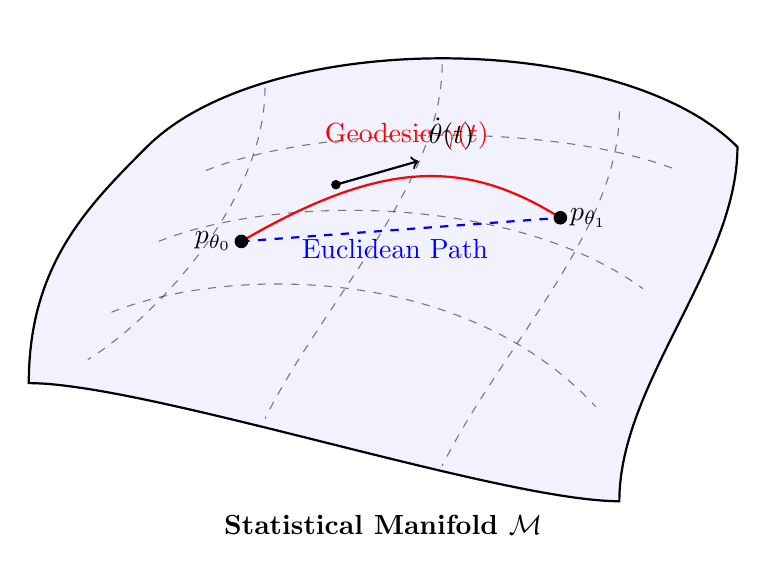
\begin{tikzpicture}[scale=1.5]
  % Draw a smooth, curved manifold surface
  \draw[thick, fill=blue!5] (0,0) .. controls (1,1) and (4,1) .. (5,0) 
    .. controls (5,-1) and (4,-2) .. (4,-3) 
    .. controls (3,-3) and (0,-2) .. (-1,-2) 
    .. controls (-1,-1) and (-0.5, -0.5) .. (0,0);

  % Draw grid lines to suggest curvature
  \draw[dashed, opacity=0.5] (0.5,-0.2) .. controls (1.5, 0.2) and (3.5, 0.2) .. (4.5,-0.2);
  \draw[dashed, opacity=0.5] (0.1,-0.8) .. controls (1.1, -0.4) and (3.1, -0.4) .. (4.2,-1.2);
  \draw[dashed, opacity=0.5] (-0.3,-1.4) .. controls (0.7, -1.0) and (2.7, -1.0) .. (3.8,-2.2);

  \draw[dashed, opacity=0.5] (1,0.5) .. controls (1,-0.5) and (0,-1.5) .. (-0.5,-1.8);
  \draw[dashed, opacity=0.5] (2.5,0.7) .. controls (2.5,-0.3) and (1.5,-1.3) .. (1,-2.3);
  \draw[dashed, opacity=0.5] (4,0.3) .. controls (4,-0.7) and (3,-1.7) .. (2.5,-2.7);

  % Points P and Q
  \coordinate (P) at (0.8,-0.8);
  \coordinate (Q) at (3.5,-0.6);

  % Draw geodesic
  \draw[thick, red] (P) .. controls (2.0, -0.1) and (2.7, -0.1) .. (Q);

  % Draw Euclidean line for contrast
  \draw[thick, blue, dashed] (P) -- (Q);

  % Labels and points
  \filldraw[black] (P) circle (1.5pt) node[left] {$p_{\theta_0}$};
  \filldraw[black] (Q) circle (1.5pt) node[right] {$p_{\theta_1}$};
  \node[red, above] at (2.2, -0.1) {Geodesic $\gamma(t)$};
  \node[blue, below] at (2.1, -0.7) {Euclidean Path};
  
  % Tangent vector
  \coordinate (M) at (1.6, -0.32);
  \draw[->, thick, black] (M) -- ++(0.7, 0.2) node[above right] {$\dot{\theta}(t)$};
  \filldraw[black] (M) circle (1pt);

  \node[font=\bfseries] at (2, -3.2) {Statistical Manifold $\mathcal{M}$};
\end{tikzpicture}
\caption{A statistical manifold $\mathcal{M}$ endowed with the Fisher metric. A straight Euclidean path in parameter space (dashed blue) does not map to the shortest informational path. The true optimal path is the geodesic $\gamma(t)$ (solid red), which minimizes cumulative KL divergence.}
\label{fig:manifold_geodesic}
\end{figure}


\section{Numerical Example: Geodesics of the Univariate Gaussian}

To build intuition, we analytically compute the geodesics for the family of univariate Gaussian distributions, parameterised by $\theta = (\mu, \sigma)$. 

The density is $p(x; \mu, \sigma) = \frac{1}{\sqrt{2\pi\sigma^2}} \exp\left( -\frac{(x-\mu)^2}{2\sigma^2} \right)$. As derived in Chapter 29, the Fisher Information Matrix for this family is diagonal:
\begin{equation}
I(\mu, \sigma) = \begin{pmatrix} \frac{1}{\sigma^2} & 0 \\ 0 & \frac{2}{\sigma^2} \end{pmatrix}
\end{equation}
The infinitesimal squared distance is given by:
\begin{equation}
ds^2 = \frac{d\mu^2 + 2d\sigma^2}{\sigma^2}
\end{equation}
Let us apply a coordinate transformation to the variance. Define $\tilde{\sigma} = \sqrt{2}\sigma$. Substituting this into the metric yields:
\begin{equation}
ds^2 = \frac{d\mu^2 + d\tilde{\sigma}^2}{(\tilde{\sigma}/\sqrt{2})^2} = 2 \frac{d\mu^2 + d\tilde{\sigma}^2}{\tilde{\sigma}^2}
\end{equation}
This metric corresponds exactly (up to a constant scaling factor of 2) to the \textit{Poincaré half-plane model} of hyperbolic geometry. The statistical manifold of univariate Gaussians is therefore a space of constant negative curvature $K = -1/2$.

In hyperbolic geometry, the geodesics are known rigorously to be either vertical lines or semicircles whose centers lie on the horizontal axis ($\tilde{\sigma} = 0$).

To verify this dynamically, we can compute the Christoffel symbols. Using $\theta^1 = \mu$ and $\theta^2 = \sigma$, the non-zero derivatives of the metric components $g_{11} = 1/\sigma^2$ and $g_{22} = 2/\sigma^2$ are:
\begin{equation}
\frac{\partial g_{11}}{\partial \sigma} = -\frac{2}{\sigma^3}, \quad \frac{\partial g_{22}}{\partial \sigma} = -\frac{4}{\sigma^3}
\end{equation}
Evaluating the Christoffel symbols gives:
\begin{equation}
\Gamma^1_{12} = \Gamma^1_{21} = -\frac{1}{\sigma}, \quad \Gamma^2_{11} = \frac{1}{2\sigma}, \quad \Gamma^2_{22} = -\frac{1}{\sigma}
\end{equation}
Substituting these into the geodesic equation yields the coupled system:
\begin{align}
\ddot{\mu} - \frac{2}{\sigma} \dot{\mu} \dot{\sigma} &= 0 \\
\ddot{\sigma} + \frac{1}{2\sigma} \dot{\mu}^2 - \frac{1}{\sigma} \dot{\sigma}^2 &= 0
\end{align}
The solutions to these differential equations precisely describe semicircular arcs parameterized by time $t$. 

Consider the implications. Suppose we wish to transition from $N(\mu_1, \sigma^2)$ to $N(\mu_2, \sigma^2)$. The Euclidean path in parameter space would simply interpolate the mean: $\mu(t) = (1-t)\mu_1 + t\mu_2$, while keeping the variance fixed at $\sigma$. However, the geodesic path dictates that we must follow a semicircle. We must first \textit{increase} the variance, shift the mean, and then \textit{decrease} the variance back to its original value. 

Information-theoretically, this is deeply satisfying. If we simply shift the mean of a highly confident (low variance) distribution, the intermediate distributions will have virtually no overlap with either the starting or ending distributions, resulting in massive spikes in relative entropy. By first increasing the variance, the model "unlearns" its specific position, widening its probability mass to overlap with the target location, allowing the mean to be shifted with minimal informational friction, before finally sharpening around the target.

\begin{figure}[htbp]
\centering
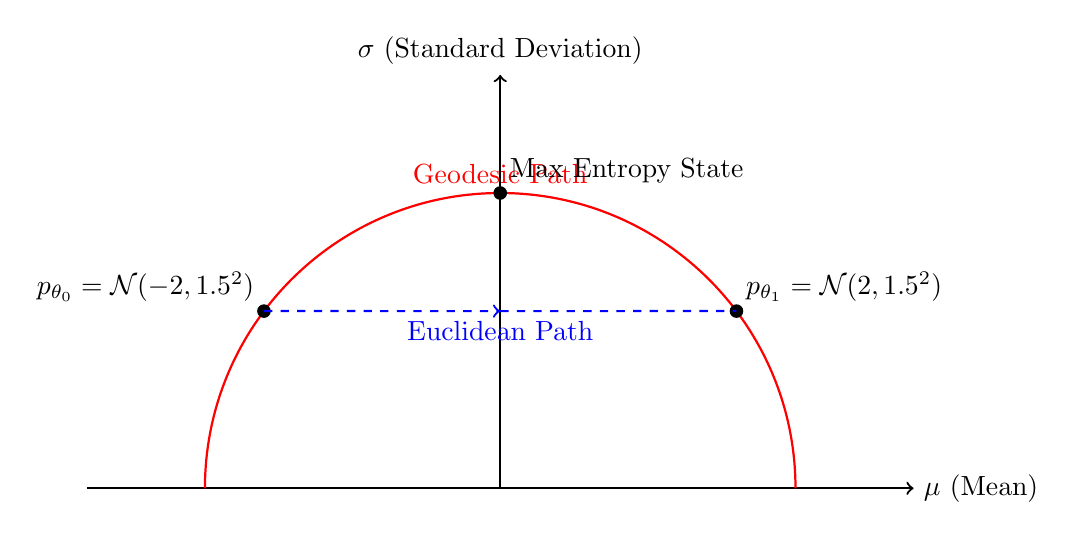
\begin{tikzpicture}[scale=1.5]
  % Axes
  \draw[->, thick] (-3.5,0) -- (3.5,0) node[right] {$\mu$ (Mean)};
  \draw[->, thick] (0,0) -- (0,3.5) node[above] {$\sigma$ (Standard Deviation)};

  % Geodesics (semicircles)
  \draw[thick, red] (2.5,0) arc (0:180:2.5);
  
  \coordinate (A) at (-2.0, 1.5);
  \coordinate (B) at (2.0, 1.5);
  
  \filldraw[black] (A) circle (1.5pt) node[above left] {$p_{\theta_0} = \mathcal{N}(-2, 1.5^2)$};
  \filldraw[black] (B) circle (1.5pt) node[above right] {$p_{\theta_1} = \mathcal{N}(2, 1.5^2)$};
  
  \draw[thick, blue, dashed, ->] (A) -- (0, 1.5);
  \draw[thick, blue, dashed] (0, 1.5) -- (B);
  \node[blue, below] at (0, 1.5) {Euclidean Path};
  
  \node[red, above] at (0, 2.5) {Geodesic Path};
  
  \filldraw[black] (0, 2.5) circle (1.5pt) node[above right] {Max Entropy State};
\end{tikzpicture}
\caption{Geodesics of the univariate Gaussian family in the $(\mu, \sigma)$ space. The geometry corresponds to the Poincaré half-plane. To move between two distributions with different means, the geodesic (red) passes through a state of increased variance. The Euclidean path (blue) keeps the variance fixed, which incurs a much higher informational cost due to the mismatch of narrow density functions.}
\label{fig:poincare_gaussian}
\end{figure}

\begin{horizon}
The mathematical certainty that shortest informational paths require intermediate states of high variance casts a fascinating light on the training trajectories of deep neural networks. It is conjectured that during the early phases of stochastic gradient descent, particularly when learning rate warmup or high momentum is utilized, the network effectively diffuses its parameters, passing through a high-entropy, high-variance state. This "unlearning" phase might not be an artifact of noisy gradients, but rather a reflection of the network implicitly discovering the geodesic path between its initialization and the optimal solution. 

Furthermore, an open question remains regarding the structure of geodesics in highly overparameterized models. In modern architectures, the Fisher Information Matrix is largely degenerate, possessing vast null spaces. This implies that the statistical manifold is not uniformly curved, but rather contains extensive "flat" submanifolds where moving the parameters incurs exactly zero change in the Kullback-Leibler divergence. It is conjectured that flat minima are physically connected by trivial geodesics within these zero-curvature valleys, allowing the model to wander freely without informational penalty.

Future work might show that architectures designed specifically to respect information geometry—perhaps by explicitly integrating geodesic equations or by utilizing natural gradient approximations like K-FAC—could bypass the arduous optimization paths currently enforced by Euclidean metrics. If we can analytically jump along geodesics across the singular manifold of neural representations, we might unlock training algorithms that converge orders of magnitude faster than current first-order methods.
\end{horizon}

\section{Summary}
\begin{itemize}
    \item The parameter space of a probability distribution family forms a \textbf{statistical manifold}, endowed with a Riemannian structure by the \textbf{Fisher Information Matrix}.
    \item \textbf{Geodesics} on this manifold represent the shortest informational paths between distributions, minimizing the local accumulation of Kullback-Leibler divergence along the trajectory.
    \item The equations governing these paths are second-order differential equations driven by \textbf{Christoffel symbols}, derived by minimizing the arc length functional via the calculus of variations.
    \item For the univariate Gaussian family, the statistical manifold is hyperbolic (the Poincaré half-plane). Geodesics are semicircles, demonstrating the counterintuitive but mathematically rigorous fact that the most efficient way to change a distribution's mean involves temporarily increasing its variance.
\end{itemize}

\section{Exercises}
\begin{enumerate}
    \item \textbf{Exponential Families and Flatness.} Prove that for an exponential family distribution parameterized by its natural parameters $\eta$, the connection induced by the Fisher Information Metric is flat, meaning all components of the Riemann curvature tensor vanish.
    \item \textbf{Distance of Bernoulli Distributions.} Compute the Fisher-Rao geodesic distance between two Bernoulli distributions with success probabilities $p_1$ and $p_2$. Show that applying the transformation $p = \sin^2(\theta)$ makes the Fisher metric Euclidean, and deduce the geodesic distance formula.
    \item \textbf{Geodesic Integration.} Write a Python script to numerically integrate the geodesic equation for a bivariate Gaussian family with a full covariance matrix. Verify computationally that the resulting trajectory minimizes the discrete accumulation of KL divergences compared to a naive linear interpolation in Euclidean parameter space.
\end{enumerate}

% TODO-CITE: Ensure all named results are cited.
